\documentclass{article}
\usepackage{listings}
\usepackage{mathrsfs}
\usepackage[utf8]{inputenc}
\usepackage{amssymb}
\usepackage{lipsum}
\usepackage{amsmath}
\usepackage{fancyhdr}
\usepackage{geometry}
\usepackage{scrextend}
\usepackage[english,german]{babel}
\usepackage{titling}
\setlength{\droptitle}{-3cm}
\usepackage{tikz}
\usepackage{algorithm,algpseudocode}
\usepackage[doublespacing]{setspace}
\usetikzlibrary{datavisualization}
\usetikzlibrary{datavisualization.formats.functions}
\usepackage{polynom}
\usepackage{amsmath}
\usepackage{gauss}
\usepackage{tkz-euclide}
\usetikzlibrary{datavisualization}
\usetikzlibrary{datavisualization.formats.functions}
\author{
Alexander Mattick Kennung: qi69dube\\
Kapitel 1
}
\usepackage{import}
\date{\today}
\geometry{a4paper, margin=2cm}
\usepackage{stackengine}
\parskip 1em
\newcommand\stackequal[2]{%
  \mathrel{\stackunder[2pt]{\stackon[4pt]{=}{$\scriptscriptstyle#1$}}{%
  $\scriptscriptstyle#2$}}
 }
\makeatletter
\renewcommand*\env@matrix[1][*\c@MaxMatrixCols c]{%
  \hskip -\arraycolsep
  \let\@ifnextchar\new@ifnextchar
  \array{#1}}
\makeatother
\lstset{
  language=haskell,
}
\lstnewenvironment{code}{\lstset{language=Haskell,basicstyle=\small}}{}
\usepackage{enumitem}
\setlist{nosep}
\usepackage{titlesec}

\titlespacing*{\subsection}{0pt}{2pt}{3pt}
\titlespacing*{\section}{0pt}{0pt}{5pt}
\titlespacing*{\subsubsection}{0pt}{1pt}{2pt}
\title{Vorlesung 4}


\begin{document}
	\maketitle
	Die Verteilungsfunktion von $\mathcal{N}(0,1)$ ($\Phi(x<X)$)  ist punktsymetrisch um (0,0.5).\\
	Also bekommt man den Wert $P(X\leq Y) = \Phi(-Y) = 1-\Phi(Y)$
	\section{Integral in $\mathbb{R}^2$}
	``gekoppelte Modelle'' aus mehreren Zufallsvariablen. Die Wahrscheinlichkeit ist jetzt definiert, als eine Funktion über diese zwei Zufallsvariablen. Im kontinuierliche ist dies ein integral über die ``Fläche'' des Integrals.\\
	\subsection{Parameterintegral}
	$I\subseteq \mathbb{R}$ sei ein Interval $f:[a,b]\times I \to \mathbb{R}$ eine Funktion $f(t,x)$ von zwei variablen $[a,b]\times I = \{(t,x)\in\mathbb{R}^2 : t\in[a,b], x\in I\}$\\
	\[F(x) = \int^b_a f(t,x)dt\]
	heißt Integralfunktion und das Integral ein Parameterintegral. (hier ist x ein parameter und nur t wird integriert)\\
	Beispiel:\\
	Gesucht ist eine Parabel p mit Scheitel im Ursprung, für die integrierte quadratische Abweichung vvon $q(x)=x^4$ im Intervall $[-1,1]$\\
	$p(x)=a\cdot x^2$, also Parameterintegral über $[-1,1]$ von da aus hat man ein normales minmierungsproblem in a.\\
	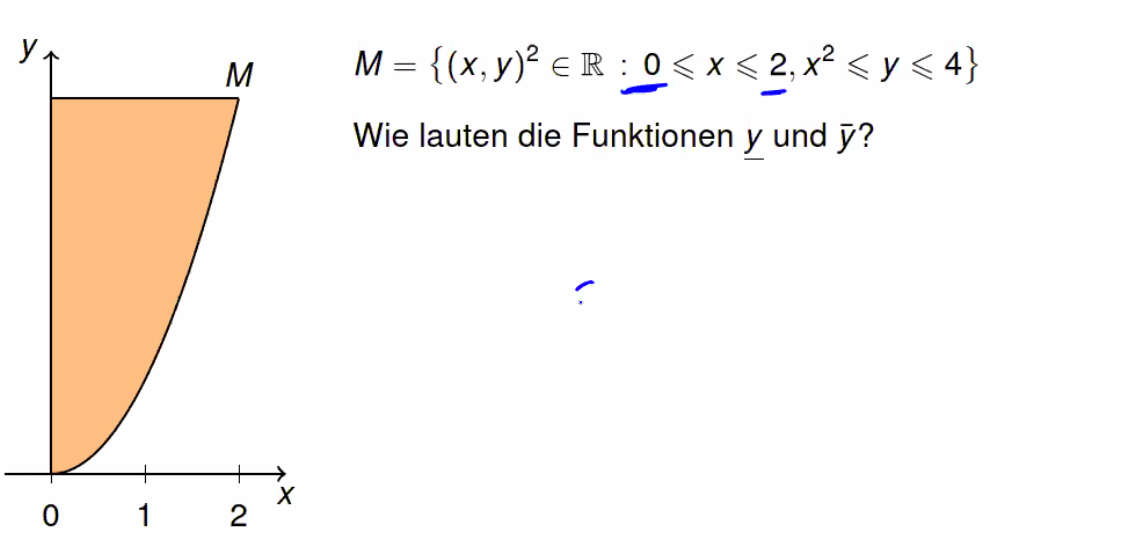
\includegraphics[width=256px]{yprojezierbarkeit.png}\\
	$\int_M f dM = \int_0^2 (\int _{\underline{y(x)}}^{\overline{y(x)}} x+y dy)dx= \int^0_2\int_{x^2}^4 x+y dy dx = \int ^2_0 [x*y+\frac{1}{2}y^2]^{y=4}_{y=x^2} dx$\\
	$=\int^2_0 (x*4+8-(x*x^2+\frac{1}{2}(x^2)^2))dx =\dots$\\
	Weiterführende Fragen:\\
	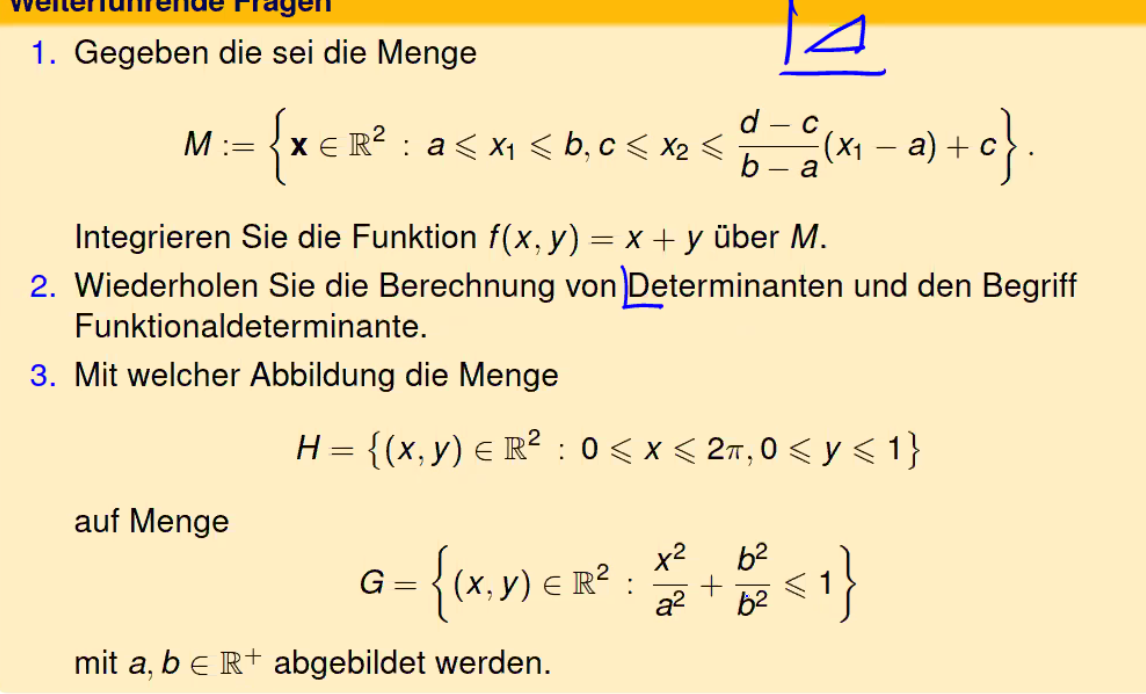
\includegraphics[width=256px]{selbststudium.png}\\
	integral $M=\{x\in\mathbb{R}^2:a\leq x_1\leq b, c\leq x_2 \leq \frac{d-c}{b-a}(x_1-a)+c\}$\\
	ist hier $x_2$ projeziert und $x_1$-projezierbar.\\
	und integrieren über $f(x,y)=1$\\
	$$\int ^b_a \int^{\frac{d-c}{b-a}(x_1-a)+c}_c 1\: dx_2dx_1 = \mu(M)$$
	wobei $\mu$ das Maß von M ist.\\
	$$\int ^b_a {\frac{d-c}{b-a}(x_1-a)+c}-c \: dx_1$$
	$$\int ^b_a \frac{d-c}{b-a}x_2-\frac{d-c}{b-a}a \: dx_1$$
	$$ (\frac{d-c}{2(b-a)}b^2-\frac{d-c}{b-a}ab)-(\frac{d-c}{2(b-a)}(a)^2-\frac{d-c}{b-a}a^2)$$
	$$ \frac{d-c}{2(b-a)}(b^2-2ab-a^2+2a^2)$$
	$$ \frac{d-c}{2(b-a)}(b-a)^2 = \frac{1}{2}(d-c)(b-a)$$
	Das integral muss so gebaut sein, dass die äußere Integrationsgrenze irgendwo im inneren integral vorkommt.\\
	Die äußeren sind die, die nicht von einer variablen abhängen:\\
	$$\int^a_b \left(\int ^{\overline{y}(x)}_{\underline{y}(x)}f(x,y)dy\right) dx$$
	Funktionaldeterminante: Determinante der jacobi-matrix $det(Jf(x))$\\
	Veralgemeinerung auf nicht-quadratische $\mathbb{R}^n\to \mathbb{R}^m$ transformationen. (liefert eine nicht quadratische jacobimatrix, mit breite= anzahl eingabe-parameter und höhe=anzahl ausgabeparameter=$\mathbb{R}^{m\times n}$)\\
	$$\mathcal{J}f(x):= \sqrt{(det((Jf(x))^TJf(x)))}$$
	3.\\
	Einfacherer Fall mit $a=b=1$: Gesucht mapping x auf Winkel, y auf radius:\\
	$x=\rho$ und $y=r$\\
	$(y*\sin(x),y*cos(x))$\\
	Jetzt wieder das a,b hinzunehmen $(a*y*\sin(x),b*y*cos(x))$ (wenn wir das einsetzen, reduziert sich das ganze auf die a/b freie variante)\\
	Die funktion ist stetig diffbar, bijektiv (ohne null), nichtlinear\\
	Daraus folgt, dass aus dem rechten Block zwei nahe Punkte auf nahe Punkte transferiert werden.\\
	Diese koordinatentransformation macht das rechnen viel einfacher: über rechteck integrieren und dann auf die ellipse abbilden.\\

\end{document}
